% Options for packages loaded elsewhere
\PassOptionsToPackage{unicode}{hyperref}
\PassOptionsToPackage{hyphens}{url}
%
\documentclass[
  11pt,
  a4paper,11pt]{article}
\usepackage{amsmath,amssymb}
\usepackage{iftex}
\ifPDFTeX
  \usepackage[T1]{fontenc}
  \usepackage[utf8]{inputenc}
  \usepackage{textcomp} % provide euro and other symbols
\else % if luatex or xetex
  \usepackage{unicode-math} % this also loads fontspec
  \defaultfontfeatures{Scale=MatchLowercase}
  \defaultfontfeatures[\rmfamily]{Ligatures=TeX,Scale=1}
\fi
\usepackage{lmodern}
\ifPDFTeX\else
  % xetex/luatex font selection
\fi
% Use upquote if available, for straight quotes in verbatim environments
\IfFileExists{upquote.sty}{\usepackage{upquote}}{}
\IfFileExists{microtype.sty}{% use microtype if available
  \usepackage[]{microtype}
  \UseMicrotypeSet[protrusion]{basicmath} % disable protrusion for tt fonts
}{}
\makeatletter
\@ifundefined{KOMAClassName}{% if non-KOMA class
  \IfFileExists{parskip.sty}{%
    \usepackage{parskip}
  }{% else
    \setlength{\parindent}{0pt}
    \setlength{\parskip}{6pt plus 2pt minus 1pt}}
}{% if KOMA class
  \KOMAoptions{parskip=half}}
\makeatother
\usepackage{xcolor}
\usepackage[margin=1in]{geometry}
\usepackage{color}
\usepackage{fancyvrb}
\newcommand{\VerbBar}{|}
\newcommand{\VERB}{\Verb[commandchars=\\\{\}]}
\DefineVerbatimEnvironment{Highlighting}{Verbatim}{commandchars=\\\{\}}
% Add ',fontsize=\small' for more characters per line
\usepackage{framed}
\definecolor{shadecolor}{RGB}{248,248,248}
\newenvironment{Shaded}{\begin{snugshade}}{\end{snugshade}}
\newcommand{\AlertTok}[1]{\textcolor[rgb]{0.94,0.16,0.16}{#1}}
\newcommand{\AnnotationTok}[1]{\textcolor[rgb]{0.56,0.35,0.01}{\textbf{\textit{#1}}}}
\newcommand{\AttributeTok}[1]{\textcolor[rgb]{0.13,0.29,0.53}{#1}}
\newcommand{\BaseNTok}[1]{\textcolor[rgb]{0.00,0.00,0.81}{#1}}
\newcommand{\BuiltInTok}[1]{#1}
\newcommand{\CharTok}[1]{\textcolor[rgb]{0.31,0.60,0.02}{#1}}
\newcommand{\CommentTok}[1]{\textcolor[rgb]{0.56,0.35,0.01}{\textit{#1}}}
\newcommand{\CommentVarTok}[1]{\textcolor[rgb]{0.56,0.35,0.01}{\textbf{\textit{#1}}}}
\newcommand{\ConstantTok}[1]{\textcolor[rgb]{0.56,0.35,0.01}{#1}}
\newcommand{\ControlFlowTok}[1]{\textcolor[rgb]{0.13,0.29,0.53}{\textbf{#1}}}
\newcommand{\DataTypeTok}[1]{\textcolor[rgb]{0.13,0.29,0.53}{#1}}
\newcommand{\DecValTok}[1]{\textcolor[rgb]{0.00,0.00,0.81}{#1}}
\newcommand{\DocumentationTok}[1]{\textcolor[rgb]{0.56,0.35,0.01}{\textbf{\textit{#1}}}}
\newcommand{\ErrorTok}[1]{\textcolor[rgb]{0.64,0.00,0.00}{\textbf{#1}}}
\newcommand{\ExtensionTok}[1]{#1}
\newcommand{\FloatTok}[1]{\textcolor[rgb]{0.00,0.00,0.81}{#1}}
\newcommand{\FunctionTok}[1]{\textcolor[rgb]{0.13,0.29,0.53}{\textbf{#1}}}
\newcommand{\ImportTok}[1]{#1}
\newcommand{\InformationTok}[1]{\textcolor[rgb]{0.56,0.35,0.01}{\textbf{\textit{#1}}}}
\newcommand{\KeywordTok}[1]{\textcolor[rgb]{0.13,0.29,0.53}{\textbf{#1}}}
\newcommand{\NormalTok}[1]{#1}
\newcommand{\OperatorTok}[1]{\textcolor[rgb]{0.81,0.36,0.00}{\textbf{#1}}}
\newcommand{\OtherTok}[1]{\textcolor[rgb]{0.56,0.35,0.01}{#1}}
\newcommand{\PreprocessorTok}[1]{\textcolor[rgb]{0.56,0.35,0.01}{\textit{#1}}}
\newcommand{\RegionMarkerTok}[1]{#1}
\newcommand{\SpecialCharTok}[1]{\textcolor[rgb]{0.81,0.36,0.00}{\textbf{#1}}}
\newcommand{\SpecialStringTok}[1]{\textcolor[rgb]{0.31,0.60,0.02}{#1}}
\newcommand{\StringTok}[1]{\textcolor[rgb]{0.31,0.60,0.02}{#1}}
\newcommand{\VariableTok}[1]{\textcolor[rgb]{0.00,0.00,0.00}{#1}}
\newcommand{\VerbatimStringTok}[1]{\textcolor[rgb]{0.31,0.60,0.02}{#1}}
\newcommand{\WarningTok}[1]{\textcolor[rgb]{0.56,0.35,0.01}{\textbf{\textit{#1}}}}
\usepackage{graphicx}
\makeatletter
\def\maxwidth{\ifdim\Gin@nat@width>\linewidth\linewidth\else\Gin@nat@width\fi}
\def\maxheight{\ifdim\Gin@nat@height>\textheight\textheight\else\Gin@nat@height\fi}
\makeatother
% Scale images if necessary, so that they will not overflow the page
% margins by default, and it is still possible to overwrite the defaults
% using explicit options in \includegraphics[width, height, ...]{}
\setkeys{Gin}{width=\maxwidth,height=\maxheight,keepaspectratio}
% Set default figure placement to htbp
\makeatletter
\def\fps@figure{htbp}
\makeatother
\setlength{\emergencystretch}{3em} % prevent overfull lines
\providecommand{\tightlist}{%
  \setlength{\itemsep}{0pt}\setlength{\parskip}{0pt}}
\setcounter{secnumdepth}{5}
% Load essential packages early
\RequirePackage{mathtools}

% Avoid microtype issues by disabling problematic features
\PassOptionsToPackage{protrusion=false, expansion=false}{microtype}

% Essential packages for graphics, tables, and code
\usepackage{graphicx}    % For including images
\usepackage{booktabs}    % For professional-looking tables
\usepackage{caption}     % For better figure and table captions
\usepackage{listings}    % For code formatting

% Hyperlinks setup - load last
\usepackage{hyperref}
\hypersetup{
    colorlinks=true,
    linkcolor=blue,
    citecolor=blue,
    urlcolor=blue,
    pdfborder={0 0 0},    % Removes boxes around links for a cleaner look
    bookmarksopen=true,   % Opens bookmarks by default
    bookmarksdepth=2      % Controls depth of bookmarks
}

% Listings configuration for code chunks
\lstset{
    basicstyle=\ttfamily\small, % Small font for better readability in code blocks
    columns=flexible,           % Adjust column spacing automatically
    breaklines=true,            % Allow line breaks in code
    showspaces=false,           % Hide spaces for cleaner appearance
    showstringspaces=false,     % Hide spaces within strings
    keepspaces=true,            % Keeps whitespace for code alignment
    frame=single,               % Adds a simple frame around code blocks
    rulecolor=\color{gray},     % Frame color for consistency
    xleftmargin=1em,            % Adds padding to the left for better readability
    xrightmargin=1em,           % Adds padding to the right
    backgroundcolor=\color[gray]{0.95}, % Subtle background for code blocks
    numbers=left,               % Line numbers on the left
    numberstyle=\tiny\color{gray}, % Styling for line numbers
    lineskip=-1pt               % Reduce line spacing within code blocks
}
\usepackage{geometry}
\geometry{a4paper, margin=1in}
\usepackage{setspace}
\onehalfspacing
\usepackage{parskip}
\setlength{\parindent}{0pt}
\hypersetup{colorlinks=true, linkcolor=blue, urlcolor=blue, citecolor=blue}
\usepackage{amsmath}
\usepackage{amssymb}
\usepackage{mathtools}
\usepackage{bm}
\usepackage{caption}
\usepackage{hyperref}
\usepackage{geometry}
\usepackage{setspace}
\ifLuaTeX
  \usepackage{selnolig}  % disable illegal ligatures
\fi
\usepackage{bookmark}
\IfFileExists{xurl.sty}{\usepackage{xurl}}{} % add URL line breaks if available
\urlstyle{same}
\hypersetup{
  pdftitle={MTHM506 - Statistical Data Modelling: Individual Project},
  pdfauthor={James R Lewis},
  hidelinks,
  pdfcreator={LaTeX via pandoc}}

\title{MTHM506 - Statistical Data Modelling: Individual Project}
\author{James R Lewis}
\date{March 2025}

\begin{document}
\maketitle

{
\setcounter{tocdepth}{2}
\tableofcontents
}
\textbf{Declaration of AI Assistance}: I have used OpenAI's ChatGPT tool
in creating this report.

AI-supported/AI-integrated use is permitted in this assessment. I
acknowledge the following uses of GenAI tools in this assessment:

\begin{enumerate}
\def\labelenumi{\arabic{enumi}.}
\tightlist
\item
  I have used GenAI tools to check and debug my code.
\item
  I have used GenAI tools to proofread and correct grammar or spelling
  errors.
\item
  I have used GenAI tools to give me feedback on a draft.
\end{enumerate}

I declare that I have referenced use of GenAI outputs within my
assessment in line with the University referencing guidelines.

\newpage

\section{Introduction}\label{introduction}

\begin{itemize}
\tightlist
\item
  \textbf{Objective:} Clearly state the aim of the analysis---to
  quantify TB risk across Brazil (2012-2014), identify socio-economic
  covariates affecting TB rates, and understand spatial, temporal, and
  spatio-temporal structures.
\end{itemize}

\begin{itemize}
\tightlist
\item
  \textbf{Relevance:} Discuss the public health importance and resource
  allocation implications.
\end{itemize}

\begin{itemize}
\tightlist
\item
  \textbf{Data Overview:} Briefly introduce the dataset, its source, and
  key variables (e.g., TB counts, socio-economic covariates, spatial and
  temporal identifiers).
\end{itemize}

\section{Exploratory Data Analysis
(EDA)}\label{exploratory-data-analysis-eda}

\begin{itemize}
\tightlist
\item
  \textbf{Descriptive Statistics:} Summarise key covariates and TB rates
  (use one table for this).
\end{itemize}

\begin{itemize}
\item
  \textbf{Visual Exploration:} Present maps or graphs that show:

  \begin{itemize}
  \item
    TB case distributions over time and across regions.
  \item
    Potential relationships between TB rates and socio-economic
    covariates.
  \end{itemize}
\end{itemize}

\begin{itemize}
\tightlist
\item
  \textbf{Spatial-Temporal Trends:} Use the provided \texttt{plot.map}
  function to visualise spatial TB distributions across years.
\end{itemize}

\section{Methodology}\label{methodology}

\begin{itemize}
\item
  \textbf{GAM Framework:}

  \begin{itemize}
  \item
    Introduce GAMs as an extension of GLMs (refer to Topic 3 notes).
  \item
    Discuss the semi-parametric nature, choice of smoothing, and
    penalisation for smoothness.
  \item
    Explain the model structure, including:

    \begin{itemize}
    \item
      Response variable: TB rate (TB cases per unit population).
    \item
      Covariates: Socio-economic factors and spatial-temporal
      indicators.
    \item
      Link function and distribution assumption (likely Poisson or
      Negative Binomial, given count data)
    \end{itemize}
  \end{itemize}
\end{itemize}

\begin{itemize}
\tightlist
\item
  \textbf{Model Formulation:} Provide the mathematical formulation of
  your GAMs, including how spatial and temporal structures are modelled.
\end{itemize}

\begin{itemize}
\tightlist
\item
  \textbf{Justification of Choices:} Explain why GAMs are appropriate,
  especially for non-linear, spatial-temporal relationships.
\end{itemize}

\section{Model Fitting}\label{model-fitting}

\begin{itemize}
\item
  \textbf{Model Development Steps:}

  \begin{itemize}
  \item
    \textbf{Initial Model:} Fit a base model with socio-economic
    covariates.
  \item
    \textbf{Spatial and Temporal Effects:} Extend the model to include
    smooth terms for spatial (latitude, longitude) and temporal (year)
    effects.
  \item
    \textbf{Spatio-Temporal Interaction:} Test for interactions if
    appropriate.
  \end{itemize}
\end{itemize}

\begin{itemize}
\tightlist
\item
  \textbf{Model Selection and Evaluation:} Discuss criteria used for
  selecting the best model (e.g., AIC, GCV, residual analysis).
\end{itemize}

\begin{itemize}
\tightlist
\item
  \textbf{Diagnostics:} Present key diagnostics (e.g., residual plots,
  deviance explained).
\end{itemize}

\section{Results}\label{results}

\begin{itemize}
\item
  \textbf{Summary of Findings:} Interpret the key model outputs:

  \begin{itemize}
  \item
    Which covariates significantly influence TB rates?
  \item
    How do spatial and temporal trends appear?
  \item
    Are there high-risk regions or periods for TB?
  \end{itemize}
\end{itemize}

\begin{itemize}
\item
  \textbf{Visual Representation:}

  \begin{itemize}
  \item
    Include maps showing predicted TB risks.
  \item
    Temporal trend plots.
  \item
    Any significant interaction effects (if modelled).
  \end{itemize}
\end{itemize}

\begin{itemize}
\tightlist
\item
  \textbf{Implications:} Discuss practical implications, particularly
  for resource allocation.
\end{itemize}

\section{Critial Review}\label{critial-review}

\begin{itemize}
\tightlist
\item
  \textbf{Model Limitations:} Reflect on any limitations (e.g.,
  assumptions, data gaps, potential overfitting).
\end{itemize}

\begin{itemize}
\tightlist
\item
  \textbf{Alternative Approaches:} Briefly discuss other modelling
  approaches that could be considered in the future.
\end{itemize}

\begin{itemize}
\tightlist
\item
  \textbf{Uncertainty Discussion:} Highlight any uncertainties in
  parameter estimation, especially regarding smooth terms.
\end{itemize}

\section{Conclusion}\label{conclusion}

\begin{itemize}
\tightlist
\item
  \textbf{Summary of Key Insights:} Recap significant findings and their
  implications.
\end{itemize}

\begin{itemize}
\tightlist
\item
  \textbf{Policy Recommendations:} Suggest actionable steps for health
  authorities based on the analysis.
\end{itemize}

\subsection{Appendix:}\label{appendix}

\begin{itemize}
\tightlist
\item
  \textbf{Commented R Code:} Include all key code used for analysis and
  modelling.
\end{itemize}

\begin{itemize}
\tightlist
\item
  \textbf{Additional Figures/Tables:} Any extra plots or results not
  included in the main text.
\end{itemize}

\begin{itemize}
\tightlist
\item
  \textbf{Model Summaries:} Full output of final model summaries.
\end{itemize}

The aim of this project is to use this data set to quantify TB risk
across Brazil over the 3 years, where risk is defined as the rate of TB
cases per unit population.

\textbf{Tables}:

\begin{enumerate}
\def\labelenumi{\arabic{enumi}.}
\tightlist
\item
  Summary Stats Table (gt table, look at website)
\item
  Model Comparison (Tweedie vs nb)
\item
  Table for regions iwth highest rate of TB, and infers from this
\end{enumerate}

\textbf{Plots}:

\begin{enumerate}
\def\labelenumi{\arabic{enumi}.}
\item
  Residual Diagnostic plots: Residual vs fitted QQ plots and 1 other?
  Influece plot?
\item
  Covariate plot 1-8 covaraite impact on rate of TB per unit pop.
  Compare the raw mean to predicted mean.
\item
  Covariate effect plot: partial effects plots to show significant
  covariates
\item
  Spatial structure explaining risk:~plot.map for this. General plot
  without temporal noise
\item
  Temporal structure explaining risk: Covariate charts/significance for
  each year
\item
  temporal-Spatial~structure explaining risk: plot.map for this. 3 of
  them, Look at differences
\end{enumerate}

The health authorities want to allocate resources for hospitals to cope
with the TB cases , so they would like to know if there are regions
where the rate of TB per unit population is high and where you would
recommend allocating these resources.

\begin{Shaded}
\begin{Highlighting}[]
 \FunctionTok{library}\NormalTok{(fields)}
\end{Highlighting}
\end{Shaded}

\begin{verbatim}
## Warning: package 'fields' was built under R version 4.4.3
\end{verbatim}

\begin{verbatim}
## Loading required package: spam
\end{verbatim}

\begin{verbatim}
## Warning: package 'spam' was built under R version 4.4.3
\end{verbatim}

\begin{verbatim}
## Spam version 2.11-1 (2025-01-20) is loaded.
## Type 'help( Spam)' or 'demo( spam)' for a short introduction 
## and overview of this package.
## Help for individual functions is also obtained by adding the
## suffix '.spam' to the function name, e.g. 'help( chol.spam)'.
\end{verbatim}

\begin{verbatim}
## 
## Attaching package: 'spam'
\end{verbatim}

\begin{verbatim}
## The following objects are masked from 'package:base':
## 
##     backsolve, forwardsolve
\end{verbatim}

\begin{verbatim}
## Loading required package: viridisLite
\end{verbatim}

\begin{verbatim}
## 
## Try help(fields) to get started.
\end{verbatim}

\begin{Shaded}
\begin{Highlighting}[]
 \FunctionTok{library}\NormalTok{(maps)}
\end{Highlighting}
\end{Shaded}

\begin{verbatim}
## Warning: package 'maps' was built under R version 4.4.3
\end{verbatim}

\begin{verbatim}
## 
## Attaching package: 'maps'
\end{verbatim}

\begin{verbatim}
## The following object is masked from 'package:purrr':
## 
##     map
\end{verbatim}

\begin{Shaded}
\begin{Highlighting}[]
 \FunctionTok{library}\NormalTok{(sp)}
\end{Highlighting}
\end{Shaded}

\begin{verbatim}
## Warning: package 'sp' was built under R version 4.4.3
\end{verbatim}

\begin{Shaded}
\begin{Highlighting}[]
 \CommentTok{\# PLotting map of cases}
 \FunctionTok{plot.map}\NormalTok{(TBdata}\SpecialCharTok{$}\NormalTok{TB[TBdata}\SpecialCharTok{$}\NormalTok{Year}\SpecialCharTok{==}\DecValTok{2014}\NormalTok{],}\AttributeTok{n.levels=}\DecValTok{7}\NormalTok{,}\AttributeTok{main=}\StringTok{"TB counts for 2014"}\NormalTok{)}
\end{Highlighting}
\end{Shaded}

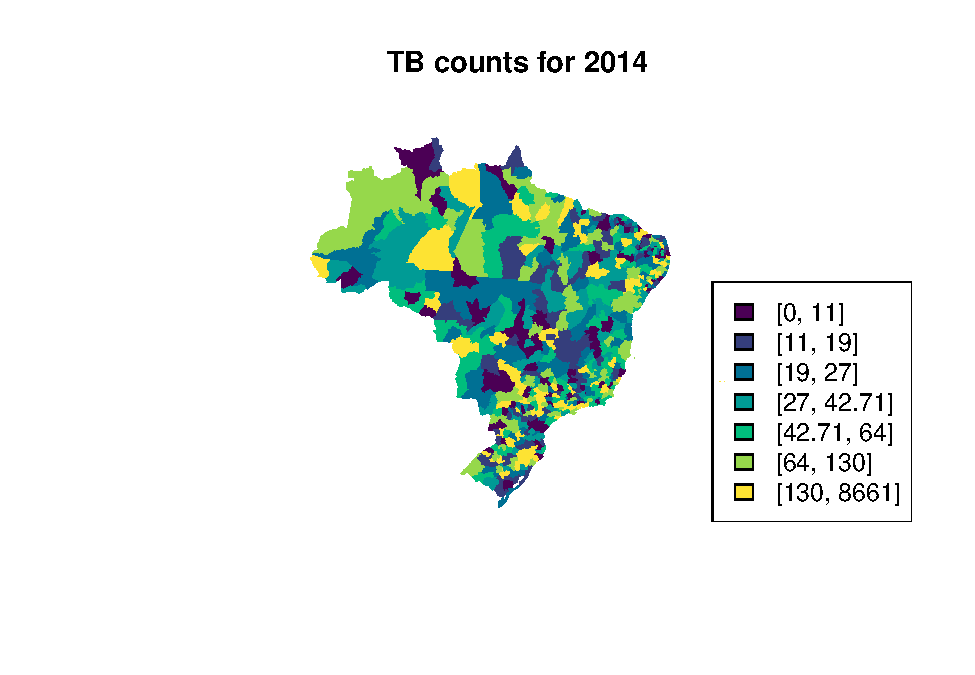
\includegraphics{Project_files/figure-latex/unnamed-chunk-1-1.pdf}

Structure:\\
\strut \\
\#\# \textbf{1. Exploratory Data Analysis (EDA)}

\begin{itemize}
\tightlist
\item
  \textbf{Descriptive Statistics:} Summary of key covariates and TB case
  rates (per unit population).
\end{itemize}

Write about Table 1

And implications going into this.

\subsection{\texorpdfstring{\textbf{2. Initial Model Fitting
(GAMs)}}{2. Initial Model Fitting (GAMs)}}\label{initial-model-fitting-gams}

\begin{itemize}
\item
  \textbf{Base Model:} Fit an initial GAM including socio-economic
  covariates.
\item
  \textbf{Model Structure Explanation:} Detail the mathematical
  formulation and rationale for including each covariate.
\item
  \textbf{Model Summary:} Present key outputs (e.g., significant
  predictors, smooth terms).
\end{itemize}

We will model \textbf{TB case counts} \(Y_{i}​\) as a function of
socio-economic covariates and spatial-temporal effects using
\textbf{Generalized Additive Models (GAMs)}. Since TB cases are
\textbf{count data}, they follow a \textbf{Poisson or Negative Binomial
(NB) distribution}, which makes the following GAM structure appropriate:

\subsection{Model Specification}\label{model-specification}

We assume that the observed TB case counts \(Y_i\) follow either a
Poisson or a Negative Binomial distribution:

\[
Y_i \sim \text{Poisson}(\mu_i) \quad \text{or} \quad Y_i \sim \text{NB}(\mu_i, \theta)
\]

where the expected mean \(\mu_i\) is modeled as:

\[
\log(\mu_i) = \beta_0 + f_1(\text{Indigenous}_i) + f_2(\text{Illiteracy}_i) + \dots + f_p(\text{Timeliness}_i) + f_{\text{spatial}}(\text{lon}_i, \text{lat}_i) + f_{\text{temporal}}(\text{Year}_i) + \log(\text{Population}_i)
\]

Here:

- \(f_j(\cdot)\) represents smooth functions capturing non-linear
effects of the socio-economic covariates.

- \(f_{\text{spatial}}(\text{lon}, \text{lat})\) models spatial
variability.

- \(f_{\text{temporal}}(\text{Year})\) accounts for temporal trends.

- The \(\log(\text{Population}_i)\) term acts as an offset to adjust for
population size.

This formulation allows us to estimate the impact of socio-economic
factors on TB case counts while incorporating spatial and temporal
structures in the data.

\subsubsection{\texorpdfstring{\textbf{Choice of Distribution: Poisson
vs.~Negative
Binomial}}{Choice of Distribution: Poisson vs.~Negative Binomial}}\label{choice-of-distribution-poisson-vs.-negative-binomial}

\paragraph{\texorpdfstring{\textbf{Limitations of the Poisson
Model}}{Limitations of the Poisson Model}}\label{limitations-of-the-poisson-model}

The Poisson model assumes that the mean and variance of the response
variable are equal:

\[
E[Y] = \text{Var}(Y)
\]

However, this assumption is often violated in real-world count data due
to \textbf{overdispersion}, where the variance exceeds the mean.
Overdispersion can lead to:

- \textbf{Inflated test statistics}, increasing the risk of Type I
errors (false positives).

\hfill\break
- \textbf{Misleading inferences}, as confidence intervals may be too
narrow.

\paragraph{\texorpdfstring{\textbf{Evidence of
Overdispersion}}{Evidence of Overdispersion}}\label{evidence-of-overdispersion}

The computed dispersion statistic for the TB data is \textbf{2223.535},
which is significantly greater than 1. This confirms severe
overdispersion, violating the equidispersion assumption of the Poisson
model:

\[
\text{Var}(Y) \gg E[Y]
\]

Using a Poisson model under such conditions would underestimate
variability, leading to unreliable statistical conclusions.

\paragraph{\texorpdfstring{\textbf{Why the Negative Binomial Model is
More
Appropriate}}{Why the Negative Binomial Model is More Appropriate}}\label{why-the-negative-binomial-model-is-more-appropriate}

The \textbf{Negative Binomial (NB) model} extends the Poisson
distribution by introducing an \textbf{overdispersion parameter}
\(\theta\), which adjusts the variance function to account for excess
dispersion:

\[
\text{Var}(Y_i) = \mu_i + \frac{\mu_i^2}{\theta}
\]

where:

- \(\mu_i\) is the expected number of TB cases for region \(i\), -
\(\theta\) controls the degree of overdispersion, allowing for greater
variability than the Poisson model.

Given the extreme overdispersion in the TB data, the Negative Binomial
model is the \textbf{statistically robust choice}, as it:

- \textbf{Relaxes the restrictive assumption of equal mean-variance}
while remaining within the exponential family framework.

- \textbf{Provides more reliable parameter estimates} by accounting for
unobserved heterogeneity across microregions.

- \textbf{Prevents misleading inference} by correcting for variance
inflation.

\paragraph{\texorpdfstring{\textbf{Justification for Directly Using a
Negative Binomial
GAM}}{Justification for Directly Using a Negative Binomial GAM}}\label{justification-for-directly-using-a-negative-binomial-gam}

Rather than initially fitting a Poisson GAM and later diagnosing
overdispersion, we \textbf{directly proceed with a Negative Binomial
GAM}. This ensures:

- \textbf{Model validity}, by selecting an appropriate variance
structure from the outset.

- \textbf{Robust inference}, reducing the risk of biased estimates and
misleading conclusions.

- \textbf{Improved accuracy}, as the model better captures the
heterogeneity in TB case counts across microregions.

By making this adjustment, we ensure a more reliable and interpretable
analysis of TB risk in Brazil.

\subsection{3. Offset for Population}\label{offset-for-population}

Since TB cases depend on the \textbf{population size} in each region, we
introduce an \textbf{offset} to model TB risk per capita:

\[
\log(\mu_i) = \text{linear predictor} + \log(\text{Population}_i)
\]

This ensures that the response variable is scaled appropriately,
effectively modeling the \textbf{rate of TB cases per 100,000 people}
rather than just raw counts.

\subsection{\texorpdfstring{\textbf{Negative Binomial GAM for TB Case
Counts}}{Negative Binomial GAM for TB Case Counts}}\label{negative-binomial-gam-for-tb-case-counts}

Given the substantial \textbf{overdispersion} in the TB case counts, we
proceed with a \textbf{Negative Binomial (NB) GAM}. The model accounts
for \textbf{spatial, temporal, and socio-economic effects} while
incorporating an \textbf{offset term} to model TB risk per unit
population.

\subsubsection{\texorpdfstring{\textbf{Mathematical
Formulation}}{Mathematical Formulation}}\label{mathematical-formulation}

The \textbf{Negative Binomial GAM} assumes that the response variable
\(Y_i\) (TB case count in region \(i\)) follows a \textbf{Negative
Binomial distribution}:

\[
Y_i \sim \text{NB}(\mu_i, \theta)
\]

where:

- \(\mu_i\) is the expected number of TB cases in region \(i\). -
\(\theta\) is the \textbf{overdispersion parameter}.

The \textbf{log link function} ensures a \textbf{multiplicative
relationship} between the covariates and the expected count:

\[
\log(\mu_i) = \beta_0 + f_1(\text{Indigenous}_i) + f_2(\text{Illiteracy}_i) + \dots + f_p(\text{Timeliness}_i) + f_{\text{spatial}}(\text{lon}_i, \text{lat}_i) + f_{\text{temporal}}(\text{Year}_i) + \log(\text{Population}_i)
\]

The \textbf{offset term} \(\log(\text{Population}_i)\) ensures that the
model accounts for diffent population sizes.

\begin{center}\rule{0.5\linewidth}{0.5pt}\end{center}

\subsection{\texorpdfstring{\textbf{Transforming Predictions to TB
Incidence
Rates}}{Transforming Predictions to TB Incidence Rates}}\label{transforming-predictions-to-tb-incidence-rates}

Since the \textbf{Negative Binomial GAM} inherently predicts \textbf{TB
case counts}, we manually convert the \textbf{fitted values} into
\textbf{TB incidence rates per 100,000 population} using:

\[
\text{Predicted TB Rate} = \left( \frac{\text{Predicted TB Cases}}{\text{Population}} \right) \times 100000
\]

This transformation ensures that the estimated values are correctly
\textbf{interpreted as TB incidence rates} rather than raw counts.

\#\#\#\#\#\#\#\#\#\#\#\#\#\#\#\#\#\#\#\#\#\#\#\#

\subsection{\texorpdfstring{\textbf{Understanding the Model
Output}}{Understanding the Model Output}}\label{understanding-the-model-output}

Even though we include an \textbf{offset term}
\(\log(\text{Population})\) in the model to account for different
\textbf{population sizes}, the model still fundamentally
\textbf{predicts TB case counts}.

\subsubsection{\texorpdfstring{\textbf{Mathematical
Formulation}}{Mathematical Formulation}}\label{mathematical-formulation-1}

The mathematical form of the model is:

\[
\log(E[Y_i]) = \beta_0 + f_1(\text{Indigenous}_i) + f_2(\text{Illiteracy}_i) + \dots + f_p(\text{Timeliness}_i) + f_{\text{spatial}}(\text{lon}_i, \text{lat}_i) + f_{\text{temporal}}(\text{Year}_i) + \log(\text{Population}_i)
\]

where: - \(E[Y_i]\) = expected \textbf{TB case count} in microregion
\(i\), - \(f_j(\cdot)\) = \textbf{smooth functions} of socio-economic
covariates, - \(f_{\text{spatial}}(\cdot)\) = \textbf{spatial effect}, -
\(f_{\text{temporal}}(\cdot)\) = \textbf{temporal effect}, -
\(\log(\text{Population}_i)\) = \textbf{offset term} to adjust for
population differences.

Since the model uses a \textbf{log link function}, the expected case
count is given by:

\[
E[Y_i] = \text{Population}_i \times e^{\text{Linear Predictor}}
\]

\subsubsection{\texorpdfstring{\textbf{Implication}}{Implication}}\label{implication}

\begin{itemize}
\tightlist
\item
  The model's predictions are in terms of \textbf{TB case counts},
  adjusted for population.
\item
  It \textbf{does not directly predict TB incidence rates}.
\item
  To obtain \textbf{TB rates}, we must \textbf{manually convert} the
  predicted case counts.
\end{itemize}

\begin{center}\rule{0.5\linewidth}{0.5pt}\end{center}

\subsection{\texorpdfstring{\textbf{2. Why Does This Happen Despite the
Offset?}}{2. Why Does This Happen Despite the Offset?}}\label{why-does-this-happen-despite-the-offset}

The \textbf{offset does not change} the response variable from
\textbf{counts to rates}. Instead, it ensures that the estimated
\textbf{case counts are proportional to the population size}.

\subsubsection{\texorpdfstring{\textbf{Key
Insights}}{Key Insights}}\label{key-insights}

\begin{itemize}
\tightlist
\item
  If two regions have the \textbf{same covariate values} but
  \textbf{different populations}, the model will predict \textbf{higher
  TB case counts} for the region with the larger population.
\item
  The offset ensures that \textbf{TB risk per person is correctly
  estimated}, but the raw predictions remain in \textbf{case counts}.
\end{itemize}

Thus, while the model \textbf{adjusts for population}, it does not
inherently provide \textbf{incidence rates}, requiring us to
\textbf{explicitly transform} the predictions.

\#\#\#\#\#\#\#\#\#\#\#\#\#\#\#\#\#\#\#\#\#\#\#\#\#\#

\subsubsection{\texorpdfstring{\textbf{Fitting the Model in
R}}{Fitting the Model in R}}\label{fitting-the-model-in-r}

We use the \texttt{mgcv} package to fit a \textbf{Negative Binomial
GAM}, specifying the \textbf{offset for population size}:

\subsection{\texorpdfstring{\textbf{3. Model Refinement and
Improvement}}{3. Model Refinement and Improvement}}\label{model-refinement-and-improvement}

\begin{itemize}
\item
  \textbf{Add Complexity:} Introduce spatial and temporal smooths to
  capture unexplained variation.
\item
  Explain why some terms are included and some not. why some are
  formatted as they as.. Illitercy seems to have no significant
  correlation as seen from a plot.
\item
  \textbf{Interaction Terms:} If necessary, test for spatio-temporal
  interactions.
\item
  \textbf{Summary Table:} Present a table comparing models (AIC,
  deviance explained, etc.) to show the progression and improvements.
\end{itemize}

\subsection{\texorpdfstring{\textbf{4. Model
Diagnostics}}{4. Model Diagnostics}}\label{model-diagnostics}

\begin{itemize}
\item
  \textbf{Residual Diagnostics:} Plot residuals to assess model fit (QQ
  plots, residual vs fitted, etc.).
\item
  \textbf{Check Assumptions:} Comment on model assumptions like
  distributional assumptions, independence, and overfitting.
\end{itemize}

\subsection{\texorpdfstring{\textbf{5. Covariate Effect Plots} (Already
created)}{5. Covariate Effect Plots (Already created)}}\label{covariate-effect-plots-already-created}

\begin{itemize}
\item
  \textbf{Effect Plots for Covariates:} Show smooth effect plots (e.g.,
  \texttt{plot.gam} in R) for key socio-economic variables to visualise
  their impact on TB risk.
\item
  \textbf{Interpretation:} Discuss how each covariate affects TB risk
  and the strength of their influence.
\end{itemize}

\subsection{\texorpdfstring{\textbf{6. Spatial and Temporal Structure
Analysis}}{6. Spatial and Temporal Structure Analysis}}\label{spatial-and-temporal-structure-analysis}

\begin{itemize}
\item
  \textbf{Spatial Smoother Visualization:} Plot the estimated spatial
  effects to identify regions with high or low TB risk.
\item
  \textbf{Temporal Smoother Visualization:} Show how TB rates have
  evolved over time.
\end{itemize}

\subsection{\texorpdfstring{\textbf{7. Geospatial
Plots}}{7. Geospatial Plots}}\label{geospatial-plots}

\begin{itemize}
\item
  \textbf{Risk Maps:} Use the \texttt{plot.map} function to produce maps
  of predicted TB risks across microregions.
\item
  \textbf{Highlight High-Risk Areas:} Identify and discuss regions with
  consistently higher TB rates.
\end{itemize}

\subsection{\texorpdfstring{\textbf{9. Model
Comparison}}{9. Model Comparison}}\label{model-comparison}

\begin{itemize}
\item
  \textbf{Performance Summary:} Compare final models based on criteria
  like AIC, deviance explained, and residual diagnostics.
\item
  \textbf{Final Model Selection:} Clearly state which model is preferred
  and why.
\end{itemize}

\subsection{\texorpdfstring{\textbf{10. Conclusion and
Recommendations}}{10. Conclusion and Recommendations}}\label{conclusion-and-recommendations}

\begin{itemize}
\item
  \textbf{Key Insights:} Summarise the main findings regarding
  socio-economic influences, spatial-temporal risks, and high-risk
  areas.
\item
  \textbf{Policy Implications:} Discuss recommendations for health
  authorities, such as where to allocate resources.
\end{itemize}

\end{document}
